\section*{MODELADO BPMN Y UML DEL SISTEMA DE GESTIÓN DE CITAS MÉDICAS}
\begin{center}
\textit{Adaptación de los ejemplos de clase al proceso de agendamiento y atención de citas}
\end{center}

\section{Criterio de adaptación}

Los materiales de referencia presentan un proceso de inventario y recepción de productos. Para este proyecto se conserva la metodología enseñada: identificar participantes, actividades, decisiones, eventos, flujos de mensaje y responsabilidades. El contenido se adapta al dominio médico, en el que participan el paciente, la clínica, recepción, el médico y caja o administración.

El proceso seleccionado para modelar es \textbf{Agendar y atender una cita médica}, porque conecta los requerimientos prioritarios del proyecto: disponibilidad del médico, registro de la cita, atención clínica, cobro y actualización de la información.

\section{Caso de uso: Gestionar cita médica}

\begin{tabularx}{\textwidth}{>{\bfseries}p{0.28\textwidth}X}
\toprule
\rowcolor{azulprincipal}\textcolor{white}{Elemento} & \textcolor{white}{Descripción}\\
\midrule
Actor principal & Recepcionista\\
Actores secundarios & Paciente, Médico y Administrador\\
Caso de uso & Gestionar cita médica\\
Objetivo & Registrar una cita sin solapamientos, confirmar la atención, registrar el resultado de la consulta y asociar el cobro correspondiente.\\
Precondiciones & El usuario debe estar autenticado; el paciente y el médico deben estar registrados; debe existir un horario disponible.\\
Resultado exitoso & La cita queda registrada y atendida o confirmada, el cobro queda asociado y la información clínica permitida se conserva.\\
Flujo alternativo & Si no existe disponibilidad, el sistema informa el conflicto y permite seleccionar otro horario.\\
\bottomrule
\end{tabularx}

\begin{figure}[htbp]
\centering
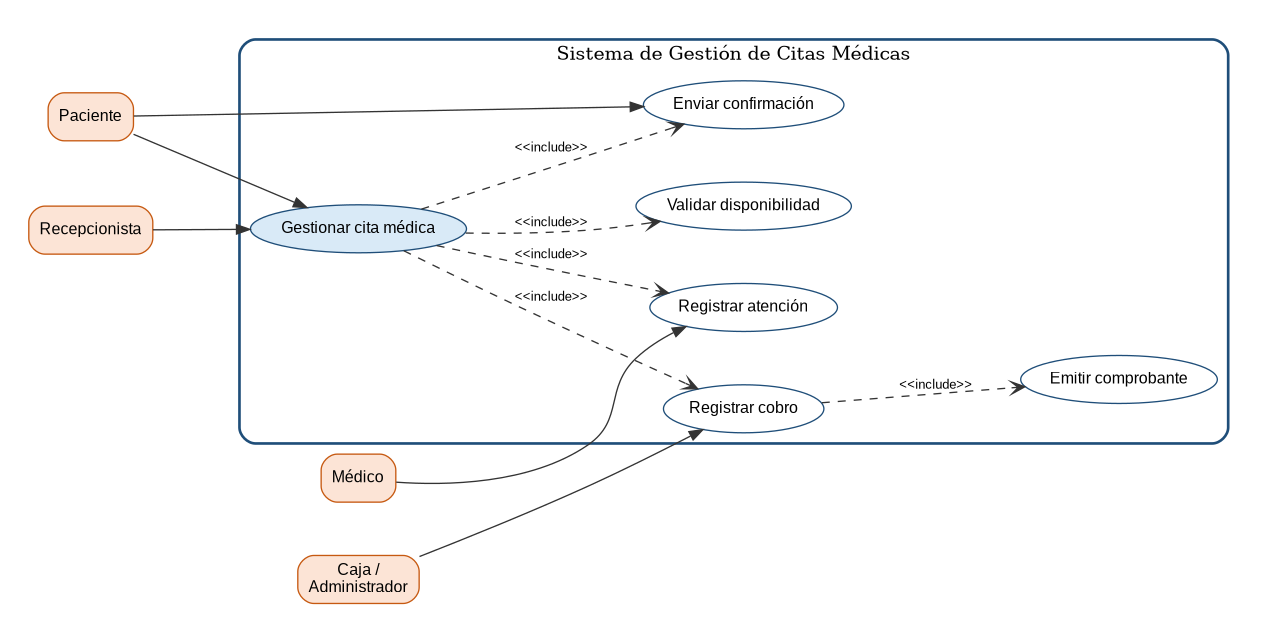
\includegraphics[width=\textwidth,height=0.50\textheight,keepaspectratio]{modelado/caso_uso_citas.png}
\caption{Caso de uso y actores de Gestionar cita médica.}
\label{fig:caso-uso-citas}
\end{figure}

\section{BPMN 2.0: Agendar y atender cita}

\subsection*{Participantes y lanes}

\begin{itemize}
    \item \textbf{Pool 1: Paciente:} solicita la cita y recibe la confirmación o el aviso de indisponibilidad.
    \item \textbf{Pool 2: Clínica:} contiene los lanes Recepción, Médico y Caja/Administración.
    \item \textbf{Lane Recepción:} registra al paciente, consulta disponibilidad y agenda la cita.
    \item \textbf{Lane Médico:} atiende la cita, registra la atención y emite una prescripción cuando corresponde.
    \item \textbf{Lane Caja/Administración:} registra el cobro, emite el comprobante y consulta reportes.
\end{itemize}

\subsection*{Flujo del proceso}

El proceso comienza cuando el paciente solicita una cita. Recepción consulta la disponibilidad del médico. La compuerta exclusiva determina si existe un horario libre: si no existe, se informa al paciente y termina el flujo alternativo; si existe, se registra y confirma la cita. En la fecha programada, el médico atiende al paciente y registra la atención. Finalmente, caja registra el cobro y genera el comprobante.

\begin{figure}[htbp]
\centering
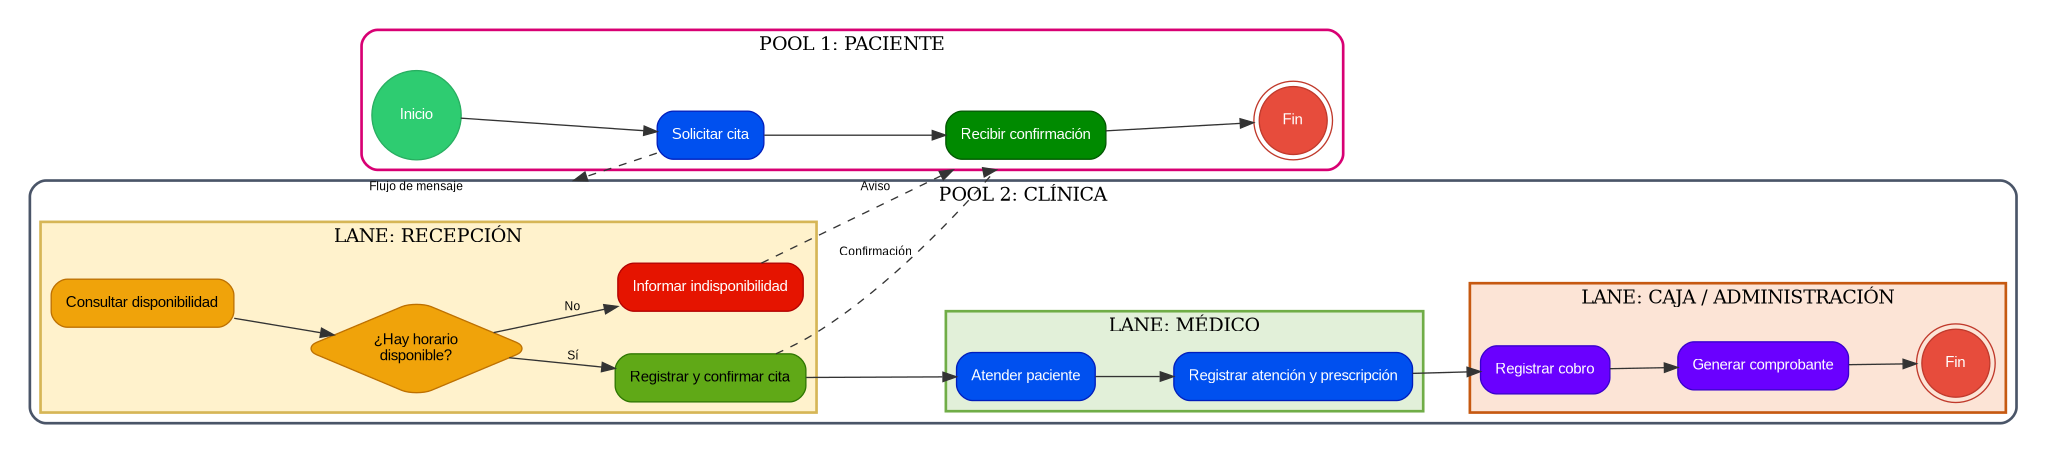
\includegraphics[width=\textwidth,height=0.50\textheight,keepaspectratio]{modelado/bpmn_citas.png}
\caption{Modelo BPMN del proceso de agendamiento y atención.}
\label{fig:bpmn-citas}
\end{figure}

\section{Diagrama de actividades UML}

El diagrama de actividades representa el flujo interno del sistema con dos responsables: Recepción y Sistema. La decisión principal es ``¿Existe disponibilidad?''. El ciclo ``¿Registrar otra cita?'' representa que el usuario puede continuar gestionando citas sin cerrar la sesión.

\begin{figure}[htbp]
\centering
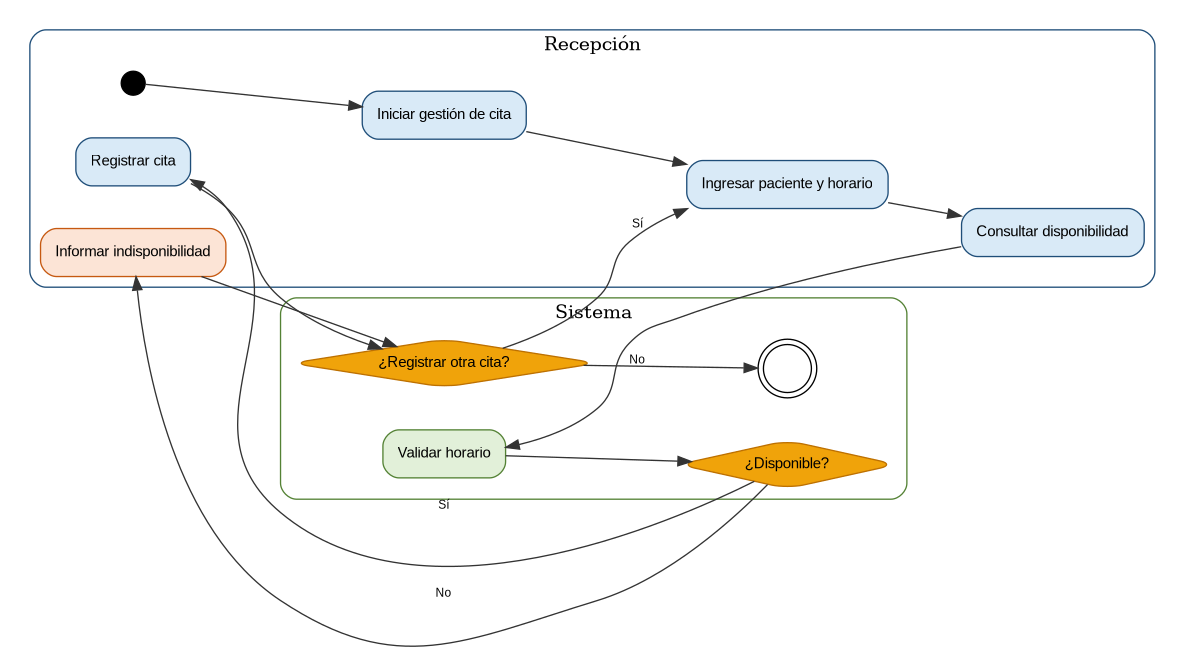
\includegraphics[width=\textwidth,height=0.50\textheight,keepaspectratio]{modelado/actividad_citas.png}
\caption{Diagrama de actividades UML para gestionar una cita.}
\label{fig:actividad-citas}
\end{figure}

\section{Diagrama de secuencia UML}

Los participantes de la interacción son Paciente, Interfaz de Citas, Gestor de Agenda, Médico, Servicio de Cobro y Base de Datos. La condición \texttt{[disponible]} permite guardar la cita; la condición \texttt{[no disponible]} devuelve un mensaje al paciente. La estructura \texttt{loop} representa la consulta o registro de varias citas durante la jornada.

\begin{figure}[htbp]
\centering
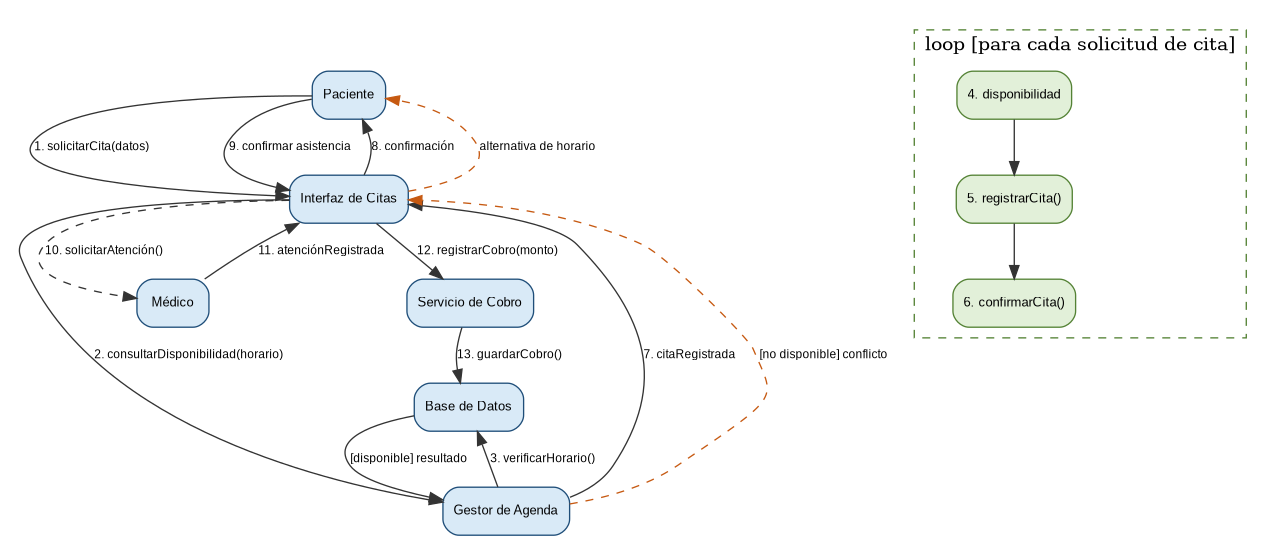
\includegraphics[width=\textwidth,height=0.50\textheight,keepaspectratio]{modelado/secuencia_citas.png}
\caption{Diagrama de secuencia UML para gestionar una cita.}
\label{fig:secuencia-citas}
\end{figure}

\section{Trazabilidad con los requerimientos}

\begin{tabularx}{\textwidth}{>{\bfseries}p{0.22\textwidth}p{0.30\textwidth}X}
\toprule
\rowcolor{azulprincipal}\textcolor{white}{Modelo} & \textcolor{white}{Requerimientos relacionados} & \textcolor{white}{Evidencia en el modelo}\\
\midrule
Caso de uso & RF-001, RF-002, RF-003 & El actor inicia la gestión, se valida la disponibilidad y se registra el cobro.\\
BPMN & RF-001, RF-002, RN-01 & Pools, lanes, flujo de mensajes y compuerta exclusiva para evitar citas solapadas.\\
Actividades UML & RF-001, RF-002 & Secuencia de tareas, decisión de disponibilidad y repetición del proceso.\\
Secuencia UML & RF-001, RF-002, RF-003, RNF-001 & Mensajes entre interfaz, gestor, médico, cobro y base de datos.\\
\bottomrule
\end{tabularx}

\subsection*{Observación técnica}

El BPMN describe la colaboración entre participantes del proceso de negocio; los diagramas UML detallan el comportamiento funcional del software. Por ello, ambos modelos se complementan y no deben sustituirse entre sí.
